
%%%%%%%%%%%%%%%%%%%%%%%%%%%%%%%%%%%%%%%%%%%%%%%%%%%%%%%%%%%%%%%%%%%%%%%%%%%%%%%%%%%%%%%%%%%%%%%%%
%
% Document:      DM  Doc Tree  
%
%%%%%%%%%%%%%%%%%%%%%%%%%%%%%%%%%%%%%%%%%%%%%%%%%%%%%%%%%%%%%%%%%%%%%%%%%%%%%%

\documentclass{article}

\usepackage{times,layouts}
\usepackage{tikz,hyperref,amsmath}
\usetikzlibrary{positioning,arrows,shapes,decorations.shapes,shapes.arrows}
\usetikzlibrary{backgrounds,calc}

\usepackage[paperwidth=31cm,paperheight=155mm,
left=-2mm,top=3mm,bottom=0mm,right=0mm,
noheadfoot,marginparwidth=0pt,includemp=false,
textwidth=30cm,textheight=50mm]{geometry}


\newcommand\showpage{%
\setlayoutscale{0.5}\setlabelfont{\tiny}\printheadingsfalse\printparametersfalse
\currentpage\pagedesign}

\hypersetup{pdftitle={DM doc tree }, pdfsubject={Documentaiton tree for LSST DM }, pdfauthor={ William O'Mullane}}


%%%%%%%%%%%%%%%%%%%%%%%%%%%%%%%%%%%%%%%%%%%%%%%%%%%%%%%%%%%%%%%%%%%%%%%%%%%%%%%%%%%%%%%%%%%%%%%%%
%
% Document:      Boxes and lines for all diagrams
%
%%%%%%%%%%%%%%%%%%%%%%%%%%%%%%%%%%%%%%%%%%%%%%%%%%%%%%%%%%%%%%%%%%%%%%%%%%%%%%

\tikzstyle{divbox}=[rectangle, rounded corners=3pt, draw=blue, top color=blue!30!white, bottom
color=white, very thick, minimum height=12mm, inner sep=3pt, text centered, text width=35mm]

\tikzstyle{arcbox}=[rectangle, rounded corners=3pt, draw=red, top color=yellow!50!white, bottom
color=white, very thick, minimum height=12mm, inner sep=2pt, text centered, text width=50mm]

\tikzstyle{psbox}=[rectangle, rounded corners=3pt, draw=red, top color=green!50!white, bottom
color=cyan, very thick, minimum height=10mm, inner sep=2pt, text centered, text width=35mm]

\tikzstyle{docbox}=[rectangle, rounded corners=3pt, draw=black, fill=cyan!50!white, 
 very thick, minimum height=12mm, inner sep=2pt,  text centered, text width=30mm]

\tikzstyle{docboxm}=[rectangle, rounded corners=3pt, draw=black, fill=red!50!white, 
 very thick, minimum height=12mm, inner sep=2pt,  text centered, text width=30mm]

\tikzstyle{gbox}=[rectangle, rounded corners=3pt, draw=orange!80!black, top color=orange!30!white,
bottom color=white, very thick, minimum height=12mm, inner sep=5pt, text badly ragged, text width=40mm]

\tikzstyle{mbox}=[rectangle, rounded corners=3pt, draw=blue, top color=cyan!50!white, bottom
color=white, very thick, minimum height=8mm, inner sep=2pt, text centered, text width=30mm]

\tikzstyle{line}=[-, thick]
\tikzstyle{sline}=[-, thick, dashed, green]
\tikzstyle{dline}=[->, thick, cyan]
\tikzstyle{tline}=[->, thick, dashed, blue]
\tikzstyle{pline}=[->, thick,  black!60!white]

\xdefinecolor{softviolet}{rgb}{0.85, 0.8, 1.0}




\begin{document}

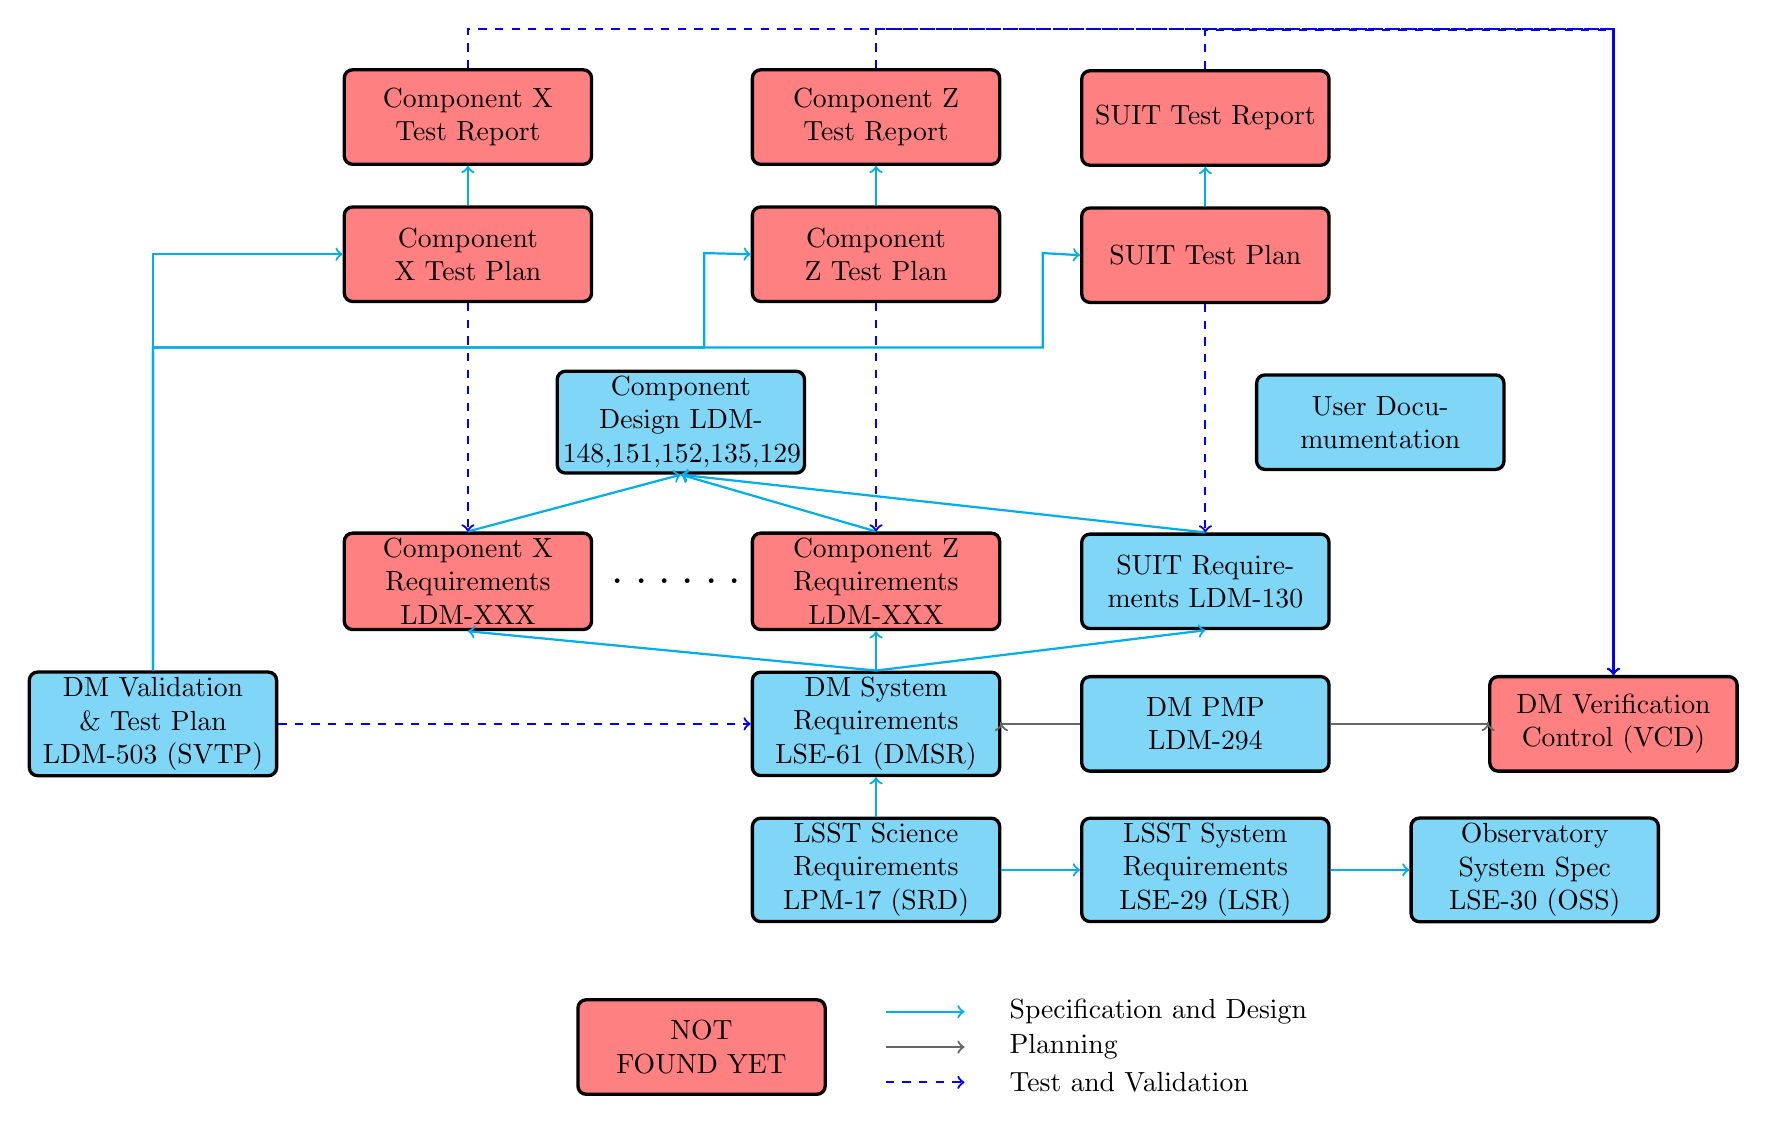
\begin{tikzpicture}[node distance=0mm]


	\node (scireq) [docbox] { LSST  Science Requirements LPM-17 (SRD)};
    \node (sysreq) [docbox, right = 1cm of scireq] { LSST  System Requirements LSE-29 (LSR)};
    \node (oss) [docbox, right = 1cm of sysreq] { Observatory System Spec LSE-30 (OSS) };
%  LEGEND
	\node(legend) [below=1cm of scireq] {};
	\node(legendr) [right=1cm of legend] {};
	\draw[dline] (legend) to (legendr);
	\node(dtext) [right= 2mm of legendr] {Specification and Design};
	\node(legend2) [below=2mm of legend] {};
	\node(legend2r) [right=1cm of legend2] {};
	\draw[pline] (legend2) to (legend2r);
	\node(ptext) [right= 2mm of legend2r] {Planning};
	\node(legend3) [below=2mm of legend2] {};
	\node(legend3r) [right=1cm of legend3] {};
	\draw[tline] (legend3) to (legend3r);
	\node(ttext) [right= 2mm of legend3r] {Test and Validation};
        \node (nf) [docboxm, left=5mm of legend2] { NOT FOUND YET };
%%%
	\node (dmreq) [docbox, above=5mm of scireq.north] { DM System Requirements  LSE-61 (DMSR)};
	\node (svtp) [docbox, left=60mm of dmreq.west] { DM  Validation \& Test Plan LDM-503 (SVTP)};
    \node (pmp) [docbox, right=10mm of dmreq.east] { DM PMP LDM-294};
    \node (vcd) [docboxm, right=20mm of pmp.east] { DM Verification Control (VCD)};

    \node (compz) [docboxm, above=5mm of dmreq.north] { Component Z Requirements LDM-XXX};
    \node (compx) [docboxm, left=20mm of compz] { Component X Requirements LDM-XXX};
    \node (crdots) [right=1mm of compx.east] {\huge \ldots \ldots};
    \node (suitr) [docbox, right=10mm of compz.east] { SUIT Requirements LDM-130};

    \node (compd)  [docbox, above=12mm of crdots] { Component Design LDM-148,151,152,135,129};
    \node (userd)  [docbox, right=5.7cm of compd] { User Documumentation };

    \node (compxt) [docboxm, above=29mm of compx] { Component X Test Plan };
    \node (compzt) [docboxm, above=29mm of compz] { Component Z Test Plan };
    \node (suitt) [docboxm, above=29mm of suitr] { SUIT Test Plan };

    \node (compxtr) [docboxm, above=5mm of compxt] { Component X Test Report };
    \node (compztr) [docboxm, above=5mm of compzt] { Component Z Test Report };
    \node (suittr) [docboxm, above=5mm of suitt] { SUIT Test Report };

   \draw[dline] (scireq.north) to (dmreq.south);
   \draw[dline] (scireq.east) to (sysreq.west);
   \draw[dline] (sysreq.east) to (oss.west);
   \draw[dline] (dmreq.north) to (suitr.south);
   \draw[dline] (dmreq.north) to (compx.south);
   \draw[dline] (dmreq.north) to (compz.south);

   \draw[dline] (svtp.north) -- ++(0,4.1)  -| ++(7,1.2) -- (compzt.west);
   
   \draw[dline] (svtp.north) -- ++(0,4.1)  -| ++(11.3,1.2) -- (suitt.west);
   \draw[dline] (svtp.north) |- (compxt.west);

   \draw[dline] (compx.north) to (compd.south);
   \draw[dline] (compz.north) to (compd.south);
   \draw[dline] (suitr.north) to (compd.south);

   \draw[tline] (suittr.north) -- ++(0,0.5)  -| (vcd.north);
   \draw[tline] (compxtr.north) -- ++(0,0.5)  -| (vcd.north);
   \draw[tline] (compztr.north) -- ++(0,0.5)  -| (vcd.north);

   \draw[tline] (svtp.east) to (dmreq.west);
   \draw[tline] (compxt.south) to (compx.north);
   \draw[tline] (compzt.south) to (compz.north);
   \draw[tline] (suitt.south) to (suitr.north);
%reports
   \draw[dline] (compxt.north) to (compxtr.south);
   \draw[dline] (compzt.north) to (compztr.south);
   \draw[dline] (suitt.north) to (suittr.south);

   \draw[pline] (pmp.west) -|  (dmreq.east);
   \draw[pline] (pmp.east) -|  (vcd.west);

   

\end{tikzpicture}
\end{document}
